\begin{figure*}[t]
\centering
\begin{subfigure}{0.62\textwidth}
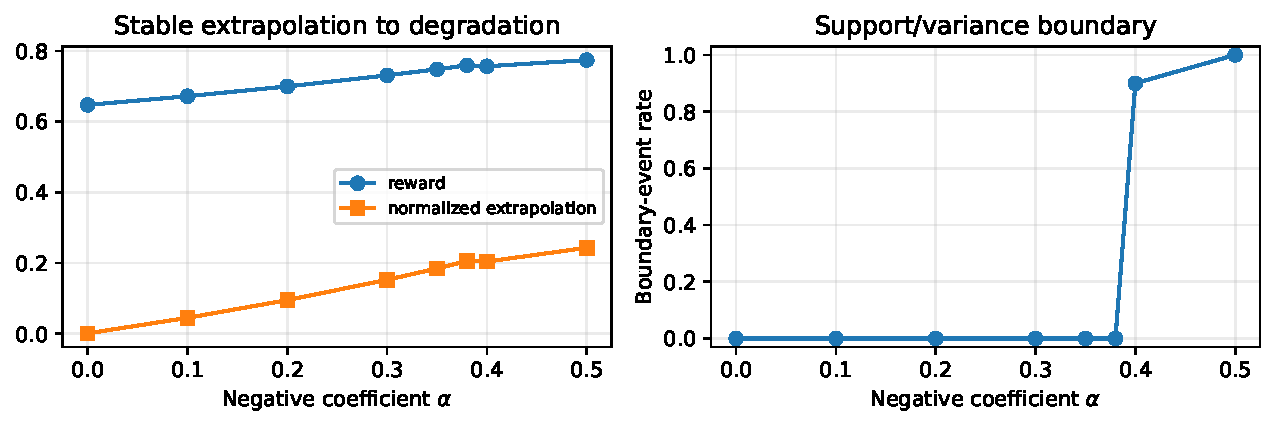
\includegraphics[width=\linewidth]{figures/generated/fig4_cu1_phase.pdf}
\caption{Strength sweep and boundary events.}
\end{subfigure}\hfill
\begin{subfigure}{0.34\textwidth}
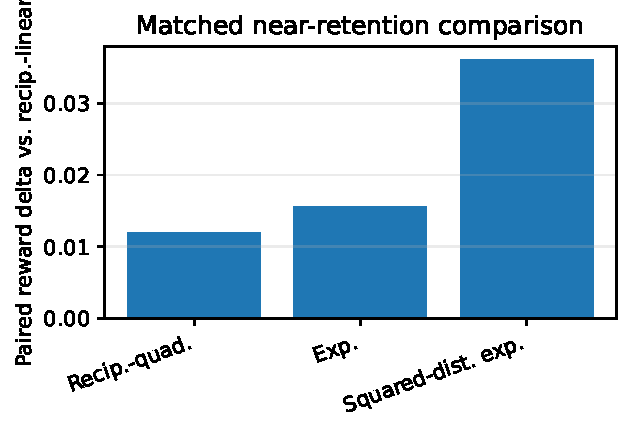
\includegraphics[width=\linewidth]{figures/generated/fig5_taper_shape.pdf}
\caption{Matched near-retention taper comparison.}
\end{subfigure}
\caption{C-U1 phase and control evidence. The strength sweep maps the transition from the Positive-only reference through stable extrapolation toward boundary events. Under the frozen near-retention protocol, all three faster-decaying tapers improve finite-horizon held-out-context reward on 20/20 paired seeds relative to reciprocal-linear; this result remains finite-step validated rather than a universal steady-state ranking.}
\label{fig:cu1-phase-control}
\end{figure*}
